% Copyright 2004 by Till Tantau <tantau@users.sourceforge.net>.
%
% In principle, this file can be redistributed and/or modified under
% the terms of the GNU Public License, version 2.
%
% However, this file is supposed to be a template to be modified
% for your own needs. For this reason, if you use this file as a
% template and not specifically distribute it as part of a another
% package/program, I grant the extra permission to freely copy and
% modify this file as you see fit and even to delete this copyright
% notice.
\documentclass[show notes]{beamer}
% There are many different themes available for Beamer. A comprehensive
% list with examples is given here:
% http://deic.uab.es/~iblanes/beamer_gallery/index_by_theme.html
% You can uncomment the themes below if you would like to use a different

%\usetheme{AnnArbor}
%\usetheme{Antibes}
%\usetheme{Bergen}
%\usetheme{Berkeley}
%\usetheme{Berlin}
%\usetheme{Boadilla}
%\usetheme{boxes}
%\usetheme{CambridgeUS}
%\usetheme{Copenhagen}
%\usetheme{Darmstadt}
%\usetheme{default}
%\usetheme{Frankfurt}
%\usetheme{Goettingen}
%\usetheme{Hannover}
%\usetheme{Ilmenau}
%\usetheme{JuanLesPins}
%\usetheme{Luebeck}
%\usetheme{Madrid}
%\usetheme{Malmoe}
%\usetheme{Marburg}
%\usetheme{Montpellier}
%\usetheme{PaloAlto}
%\usetheme{Pittsburgh}
%\usetheme{Rochester}
%\usetheme{Singapore}
%\usetheme{Szeged}
%\usetheme{Warsaw}
%\usetheme[]{metropolis}

\title{A Lagrangian geography of the deep\\Gulf of Mexico}

% A subtitle is optional and this may be deleted
%\subtitle{Optional Subtitle}

\author{Philippe Miron\inst{1},  Francisco J. Beron-Vera\inst{1}, Mar\'ia J. Olascoaga\inst{1} and Gary Froyland\inst{2}}

\institute
{
  \inst{1}%
  RSMAS University of Miami, Miami, USA
  %\and
  %\inst{2}%
  %RSMAS/OCE University of Miami, Miami, USA
  \and
  \inst{2}%
  University of New South Wales, Sydney, Australia
  }
% - Use the \inst command only if there are several affiliations.
% - Keep it simple, no one is interested in your street address.

\date{RAUGM on Thursday, October 24 2017}
%\date{2017 Oil Spill and Ecosystem Science Conference}
% - Either use conference name or its abbreviation.
% - Not really informative to the audience, more for people (including
%   yourself) who are reading the slides online

\subject{Applied oceanography}
% This is only inserted into the PDF information catalog. Can be left
% out. 

% Beamer settings
\setbeamertemplate{navigation symbols}{} %remove nav symbols
\setbeamertemplate{bibliography item}{}
\setbeamertemplate{footline}[frame number]

% If you have a file called "university-logo-filename.xxx"
% is a graphic format that can be processed by latex or pdflatex,
% resp., then you can add a logo as follows:
%\pgfdeclareimage[height=1.5cm]{logo}{figures/GoMRi.png}
%\logo{\pgfuseimage{logo}}

% Delete this, if you do not want the table of contents to pop up at
% the beginning of each subsection:
%\AtBeginSubsection[]
%{
%  \begin{frame}<beamer>{Outline}
%  \tableofcontents[currentsection,currentsubsection]
%  \end{frame}
%}

% graphic
\graphicspath{{"2017. deep floats (raugm)/figures/"}}
%\graphicspath{{"figures/"}}

% titlepage logo
\titlegraphic{
\begin{tikzpicture}[overlay, remember picture]
\node[at=(current page.south west), anchor=south west] {%
 
\includegraphics[height=.10\textwidth]{carthe.png} 
};
\node[at=(current page.south), anchor=south] {%
 
\includegraphics[height=.13\textwidth]{cigom.jpg} 
};
\node[at=(current page.south east), anchor=south east] {
 
\includegraphics[height=.10\textwidth]{um-rsmas.png}
};
\end{tikzpicture}
}

% bibliography
\usepackage[style=authoryear, natbib=true]{biblatex}
\addbibresource{fot.bib}

% remove annoying biblatex bug/warning
\usepackage{silence}
\WarningFilter{biblatex}{Patching footnotes failed}

% some definitions
\usepackage[utf8]{inputenc}
\usepackage[english]{babel}
\usepackage{amssymb}
\usepackage{amsfonts}
\usepackage{amsmath}
\usepackage{bbold}
\usepackage{ragged2e} % justify text in all frame
\apptocmd{\frame}{}{\justifying}{}
\usepackage{etoolbox}
\usepackage{tikz}
\usepackage{subfig}
\usepackage{multicol}
\usepackage{siunitx}
\usepackage{csquotes}
\usepackage{hyperref}
\usepackage{tikz,pgfplots}
\pgfplotsset{compat=1.12}

% Definitions.
\def\vol{\mathop{\rm area}}

\newcommand{\PF}{\mathcal{P}}
\newcommand{\ia}{\textit{a}}
\newcommand{\ib}{\textit{b}}
\newcommand{\ic}{\textit{c}}
\newcommand{\id}{\textit{d}}
\newcommand{\ie}{\textit{e}}
\newcommand{\gom}{GoM}
\let\vaccent=\v 
\renewcommand{\v}[1]{\ensuremath{\mathbf{#1}}} 
\newcommand{\minus}{\scalebox{0.5}[1.0]{$-$}}

% Let's get started
\begin{document}

\frame[plain,noframenumbering]{
\titlepage
}

\iffalse
\begin{frame}{Outline}
  \tableofcontents
  % You might wish to add the option [pausesections]
\end{frame}
\fi

\section{Introduction}

\frame{\frametitle{Introduction}
Over the last twenty five years, many satellite-tracked surface drifters sampled the surface of the Gulf of Mexico (\gom). From a database of 3300 drifters, we presented a Lagrangian geography of the \gom.

\begin{figure}
    \centering
    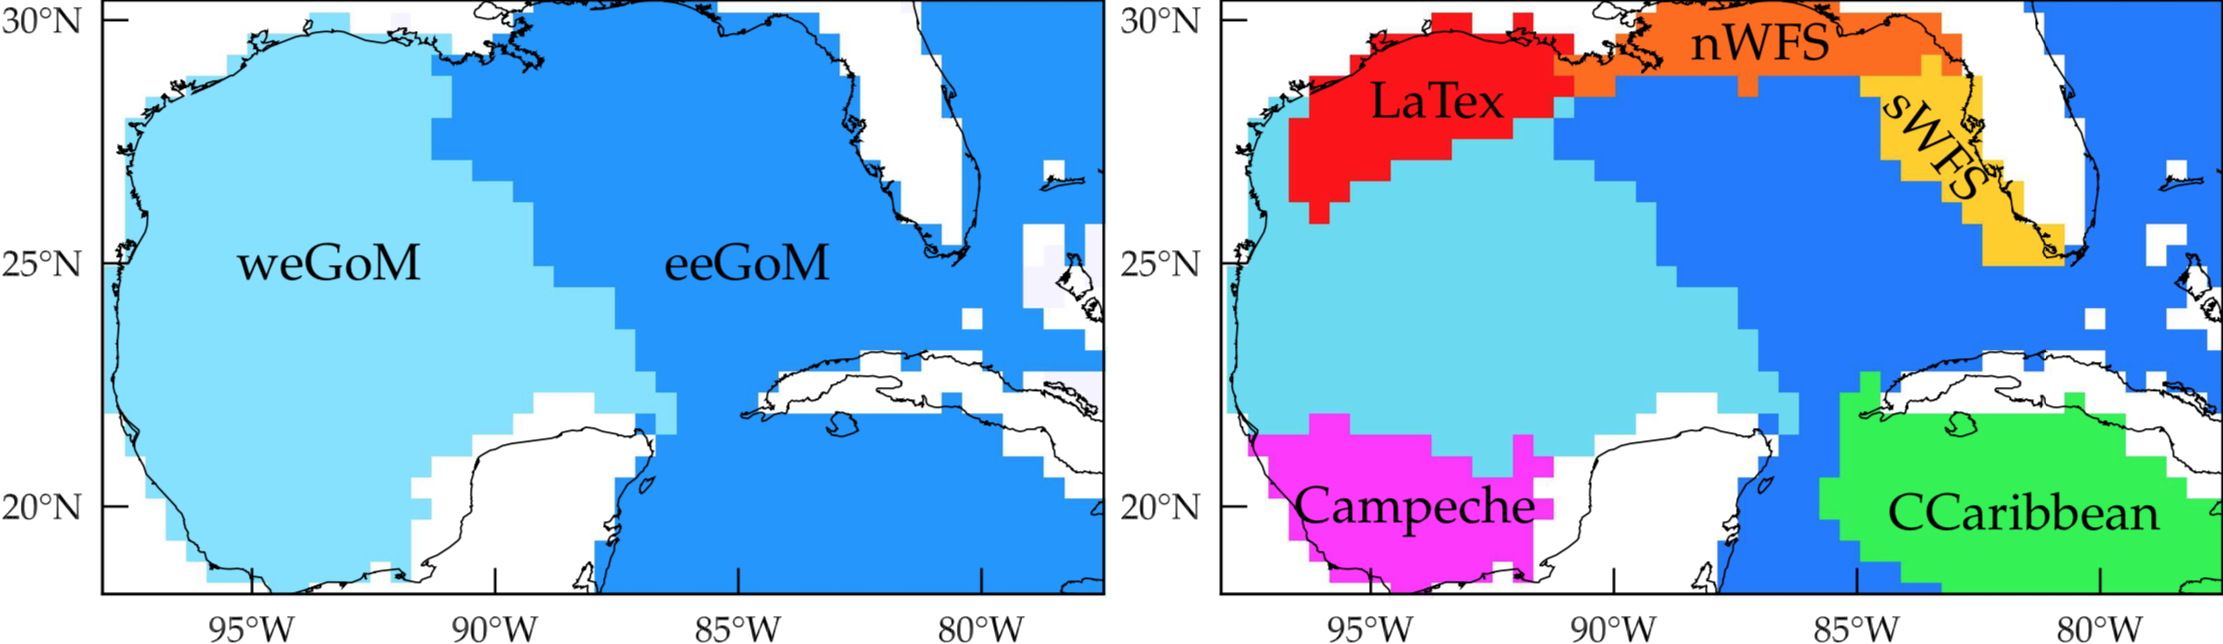
\includegraphics[width=\textwidth]{geosurf.png}
    \caption{Published in \cite{miron2017lagrangian}}
    \label{fig:geosurf}
\end{figure}
}

\frame{\frametitle{Introduction}
In contrast, very few studies were aimed at the characterization of the deep water global circulation. 
\newline\newline
RAFOS experiments sponsored by the Bureau of Ocean Energy Management (BOEM) (July 2011 - May 2015) courtesy Alexis Lugo Fernandez:
\begin{itemize}
\item 121 floats at 1500\,m
\item 31 floats at 2500\,m
\item 4-year mission (floats $\sim 2$-y mission and are redeployed)
\end{itemize}
}

\section{Objectives}

\frame{\frametitle{Objectives}
Using floats data (trajectories) in the abyssal Gulf of Mexico (\gom):
\begin{itemize}
    \item subdivide the deep \gom\ into regions with similar dynamics;
    \item identify sinks and sources (attractors and basins of attraction);
    \item predict transport of \textit{passive tracers}.
\end{itemize}
}

% Section and subsections will appear in the presentation overview
% and table of contents.
\frame{\frametitle{Theory: flowmap $F$}
Given the drifter paths, we wish to access the map $x \mapsto F(x)$ that determines how the drifters change positions. 
\newline\newline
If the ocean flow was stationary in some statistical sense, then the velocity could be express has $v(x)$.  If this case, we could simply solve the ODE $\dot{x} = v(x)$ to get $F$, the flow map, and \emph{move around} any function, such has a tracer distribution $f(x)$.
}

\frame{\frametitle{Theory: transfer operator $\mathcal{P}$}
This is done by composing $f$ with $F^{-1}$ and it defines a transfer operator $\mathcal{P}$ as the linear operator such that
\begin{equation}
    \mathcal{P}\!f(x) = f \circ F^{-1}(x).
\end{equation}

\only<2>{
Why $F^{-1}$? Example, if $F$ moves the distribution 2 units to the right.
\begin{figure}[!ht]
\centering
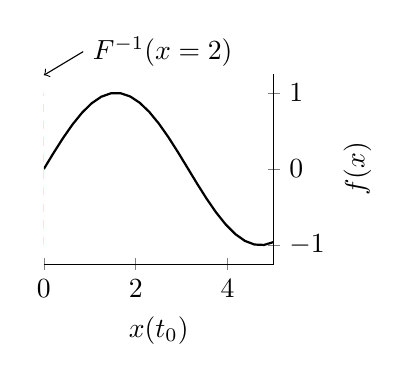
\begin{tikzpicture}
% plot curve at t0
\begin{axis}[
width=4.5cm,
height=4cm,
xmin=0, xmax=5,
ymin=-1.25, ymax=1.25,
ylabel={$f(x)$},
xlabel={$x (t_0)$},
axis y line=right,
axis x line=bottom,
axis line style={-}
]
\addplot[domain=0:5,thick]{sin(deg(x))};
\draw[dashed,color=red] (0,-1) -- (0,1);
\end{axis}
\draw [<-] (0,2.4) -- (0.5, 2.7) node[right] {$F^{-1}(x=2)$};
\end{tikzpicture}\hspace{0.25cm}
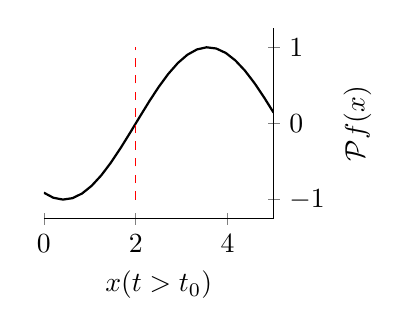
\begin{tikzpicture}
% plot curve at t0+t
\begin{axis}[
width=4.5cm,
height=4cm,
xmin=0, xmax=5,
ymin=-1.25, ymax=1.25,
ylabel={$\mathcal{P}f(x)$},
xlabel={$x (t > t_0)$},
axis y line=right,
axis x line=bottom,
axis line style={-}
]
\addplot[domain=0:5,thick]{sin(deg(x-2))};
\draw[dashed,color=red] (2,-1) -- (2,1);
\end{axis}
\end{tikzpicture}
\end{figure}
}

}

\frame{\frametitle{Theory: transfer operator $\mathcal{P}$}
For $F$ representing a non-autonomous flow as above, $\mathcal P
\!f(x)$ is the solution of
\begin{equation}
  \partial_t\rho + v\cdot\nabla\rho = 0,\quad
  \rho(x,t = 0) = f(x).
\end{equation}

In our case, \underline{$F$ is unknown} and we \underline{only have access to trajectories}. We will use a discrete method to approximate $\mathcal{P}$.
}

\frame{\frametitle{Theory: transition matrix}  
Partition the domain into equal-size bins $\{B_i,\cdots,B_N\}$ (a regular grid) and consider the indicator function of set $B_i$: 
 \begin{equation} 
	\mathbf{1}_{B_i}(x) =
  \begin{cases}
    1  & \text{if } x \in B_i,\\
    0  & \text{if } x \notin B_i.
  \end{cases}
\end{equation} 

Note that $V_N := \{\mathbf{1}_{B_1}(x),\cdots,\mathbf{1}_{B_N}(x)\}$ is a discrete orthornormal basis w.r.t. the inner product
\begin{equation}
    \langle \bullet, \mathbf 1_{B_i}(x)\rangle = \frac{1}{\vol(B_i)}\int_{B_i} \bullet\, \mathbf 1_{B_i}(x)\,d^2x = \overline{(\bullet)}^{B_i}.
\end{equation}

Then, project $f(x)$ on the basis $V_N$, called Ulam basis \citep{ulam1960}:
\begin{equation}
    \Pi_Nf(x) = \sum_1^N f_i \mathbf 1_{B_i}(x),\quad f_i = \langle f(x), \mathbf 1_{B_i}(x)\rangle = \overline{f(x)}^{B_i}
\end{equation}
where $\Pi_N$ is the projector.
}

\frame{\frametitle{Theory: how to construct the transition matrix}  
In a similar manner one can project $\mathcal P$ on $V_N$:
\begin{align}
(\Pi_N\mathcal{P})_{ij} &=  \frac{1}{\vol(B_j)}
\int_{B_j} \mathcal P \mathbf 1_{B_i}(x) \cdot
\mathbf 1_{B_j}(x)\,d^2x\nonumber\\ 
&= \frac{\vol(B_i \cap F^{-1}(B_j))}{\vol(B_i)} =: P_{ij}.
\end{align}
The entries of $P$ can be viewed as transitional probabilities of moving from $B_i$ to $B_j$ (Markov Chain with bins $\equiv$ states):
\begin{equation}
   P_{ij} = \frac{\#\text{ of particles in }B_i\text{ that are mapped to }B_j}{\#\text{ of particles in }B_i}.
  \label{eq:Pnum}
\end{equation}
}

\frame{\frametitle{Theory: transition matrix}  
$P_{ij}$ gives us the action of $F$ at a coarse-grained level given by the partition. This introduces diffusion proportional to the size of $B_i$ and is solution of: 
\begin{equation}
  \partial_t\rho + v\cdot\nabla\rho =
  D\nabla^2\rho \quad \text{with }
  \rho(x,t = 0) = f(x),
\end{equation}
with $D \propto \vol(B_i)$.
}

\frame{\frametitle{Application of the transition matrix}
One can push forward discrete representations of $f(x)$:
\begin{equation}
    \mathbf f = (f_1,\cdots,f_N),
\end{equation}
by right-multiplication by $P$:
\begin{align}
    f^{(1)} &= f\,P \nonumber\\
    f^{(2)} &= f^{(1)}\,P = f\,P^2 \nonumber\\
    f^{(k)} &= f\,P^k
\end{align}

Similarly, we push backward an initial distribution using $P^\top$.
}

\frame{\frametitle{Eigenvectors analysis}

It is also of interest to identify when a distribution $\mathbf f$ is almost invariant:
\begin{equation}
    \mathbf f \approx \mathbf f\,P
\end{equation}

This is available from the \emph{eigenspectrum} inspection of $P$ \citep{Froyland-etal-12}.
\newline\newline
If in the matrix $P$:
\begin{itemize}
    \item all states \emph{communicate};
    \item no state occurs \emph{periodically}.
\end{itemize}
$P$ has a limiting distribution $\mathbf{p} = \mathbf{p} P$.
\newline\newline
Note: $\mathbf{p}$ is a left eigenvector of $P$ with eigenvalue $\lambda = 1$ ($\mathbf{p} \lambda = \mathbf{p} P$). Because of row-stochasticity of $P$, the corresponding right eigenvector is $\mathbb{1}$, i.e., $P\mathbb{1} = \mathbb{1}$.
}

\frame{\frametitle{Attractors and basin of attractions}
Any distribution $f_\mathbb{1}$ supported on the right eigenvector $\mathbb{1}$ will converge to $\mathbf{p}$ as the number of applications of $P$ tends to infinity, i.e., $\smash{\lim_{n \to \infty} f_\mathbb{1}P^n = \mathbf{p}}$.
\newline\newline
For $\lambda = 1$:
\begin{itemize}
    \item right eigenvector of $P$ is the basin of attraction
    \item left eigenvector of $P$ is the attractor
\end{itemize}

This motivates the idea that regions where trajectories converge and their basins of attraction are encoded in the eigenvectors of the transition matrix $P$ with eigenvalues ($\lambda \approx 1$) \citep{froyland2014well}.
}


\frame{\frametitle{Data}
Trajectories of the RAFOS cover the area under 1500\,m of the Gulf of Mexico.
\begin{figure}
  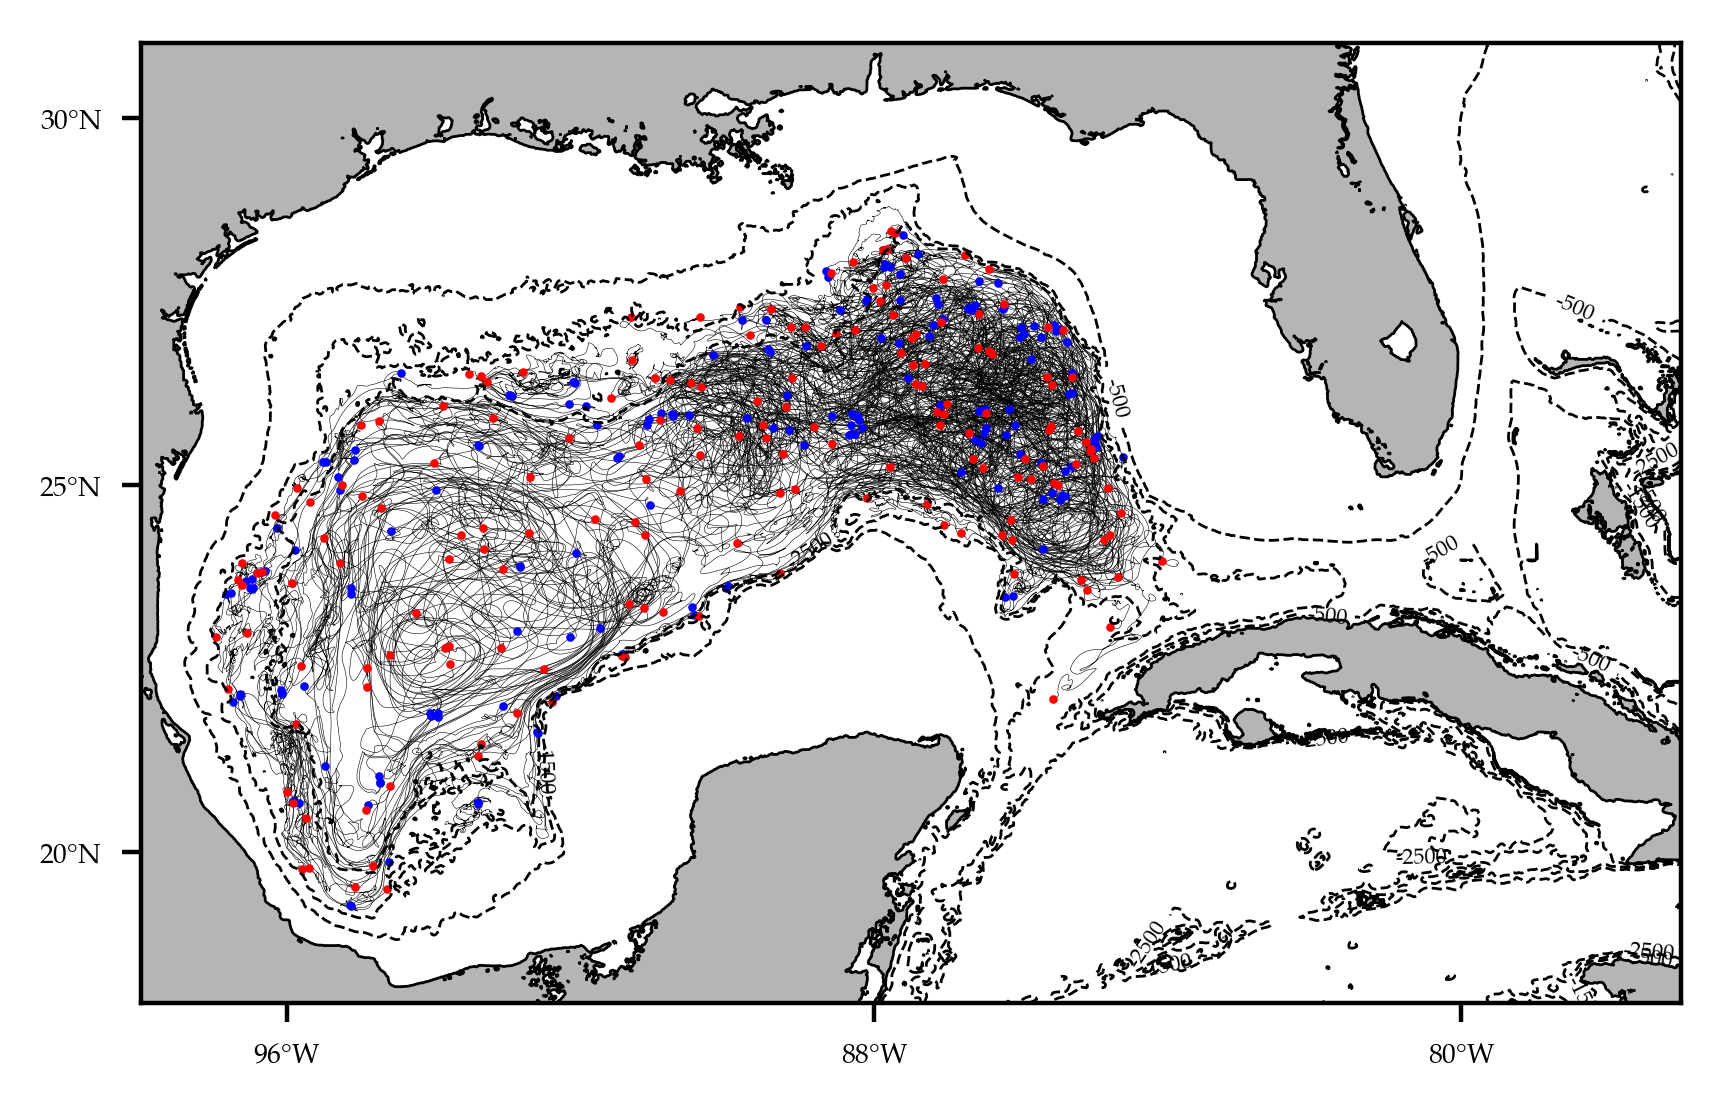
\includegraphics[width=\textwidth]{float_t0_ss.png}
\end{figure}
}


\section{Results}

\frame{\frametitle{Eigenvectors}

\only<1>{
Eigenvectors associated with $\lambda_1=1$ and $\lambda_2=0.9953$.
\begin{figure}
  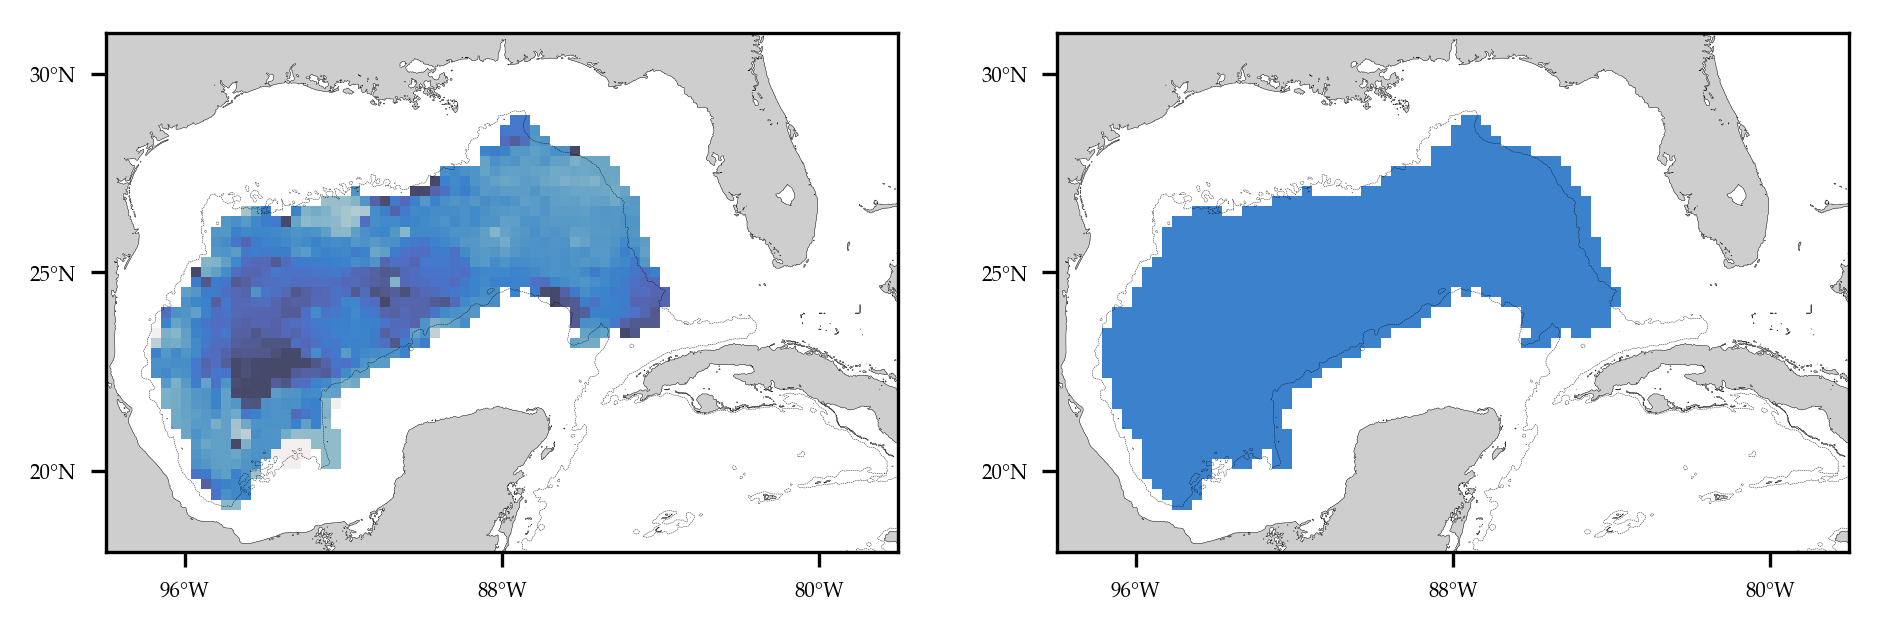
\includegraphics[width=\textwidth]{eig_QP0.png}
\end{figure}
\begin{figure}
  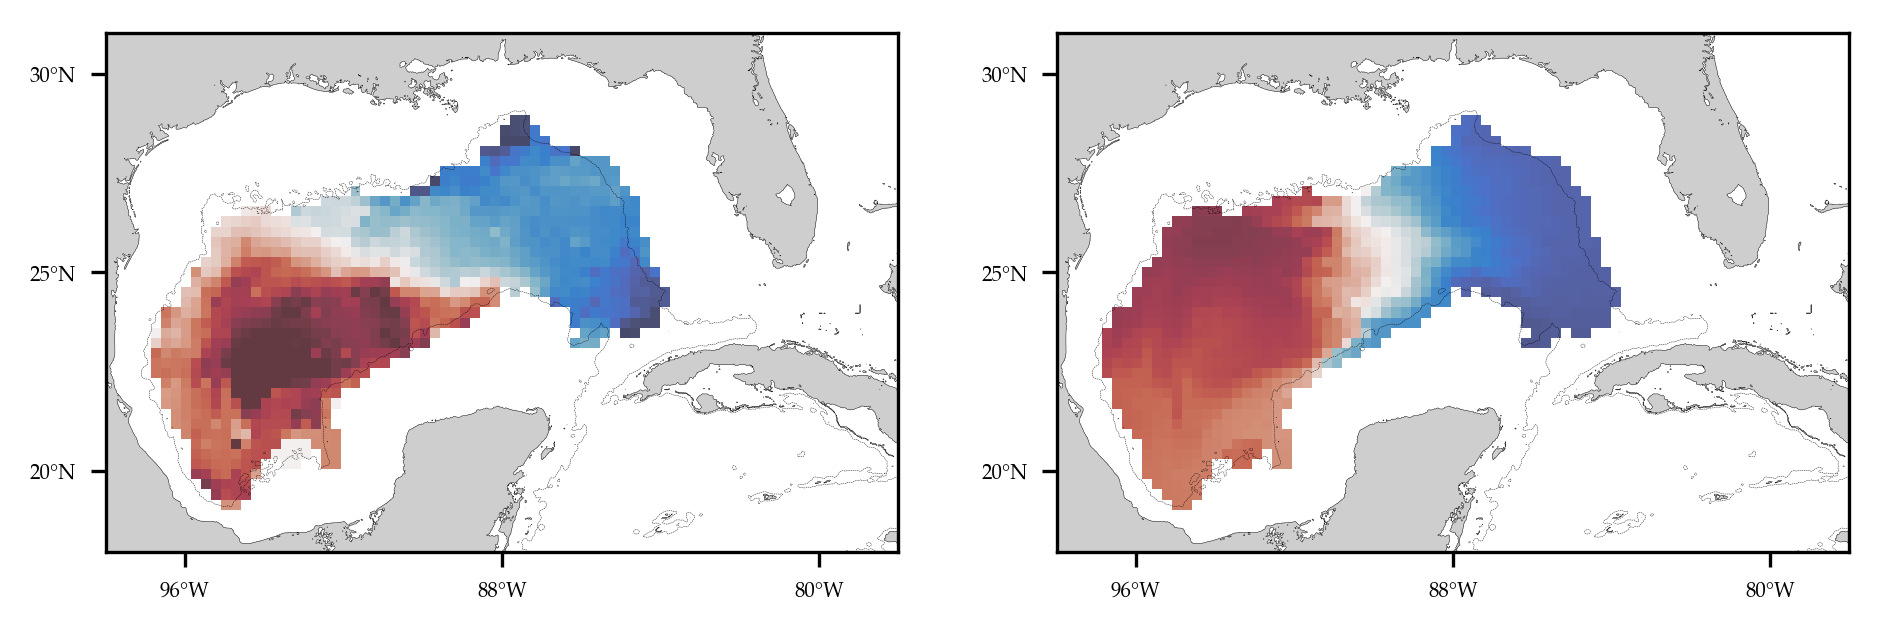
\includegraphics[width=\textwidth]{eig_QP1.png}
\end{figure}
}

\only<2>{
Eigenvectors associated with $\lambda_3=0.9832$ and $\lambda_5=0.9712$.
\begin{figure}
  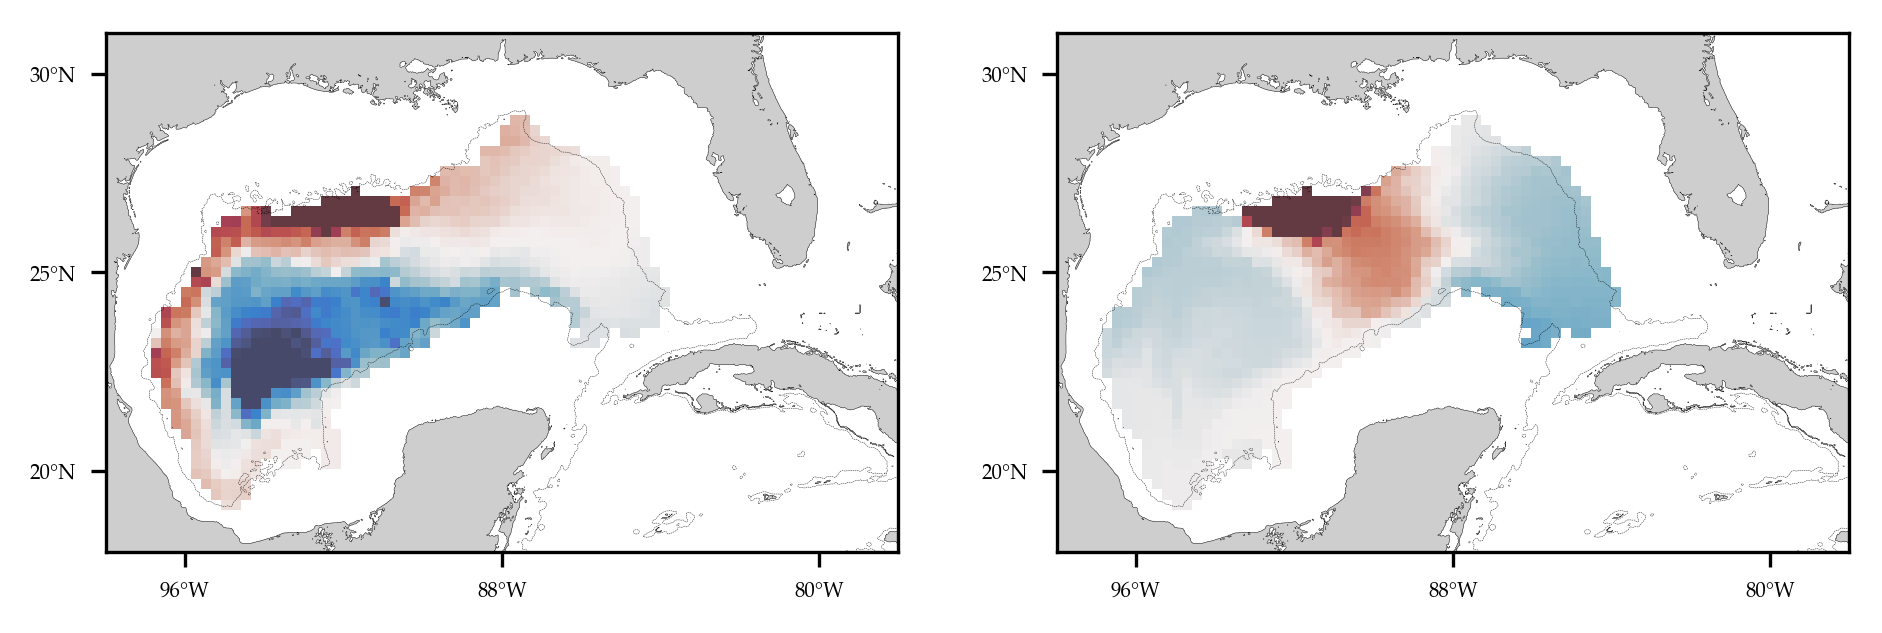
\includegraphics[width=\textwidth]{eig_QP2.png}
\end{figure}
\begin{figure}
  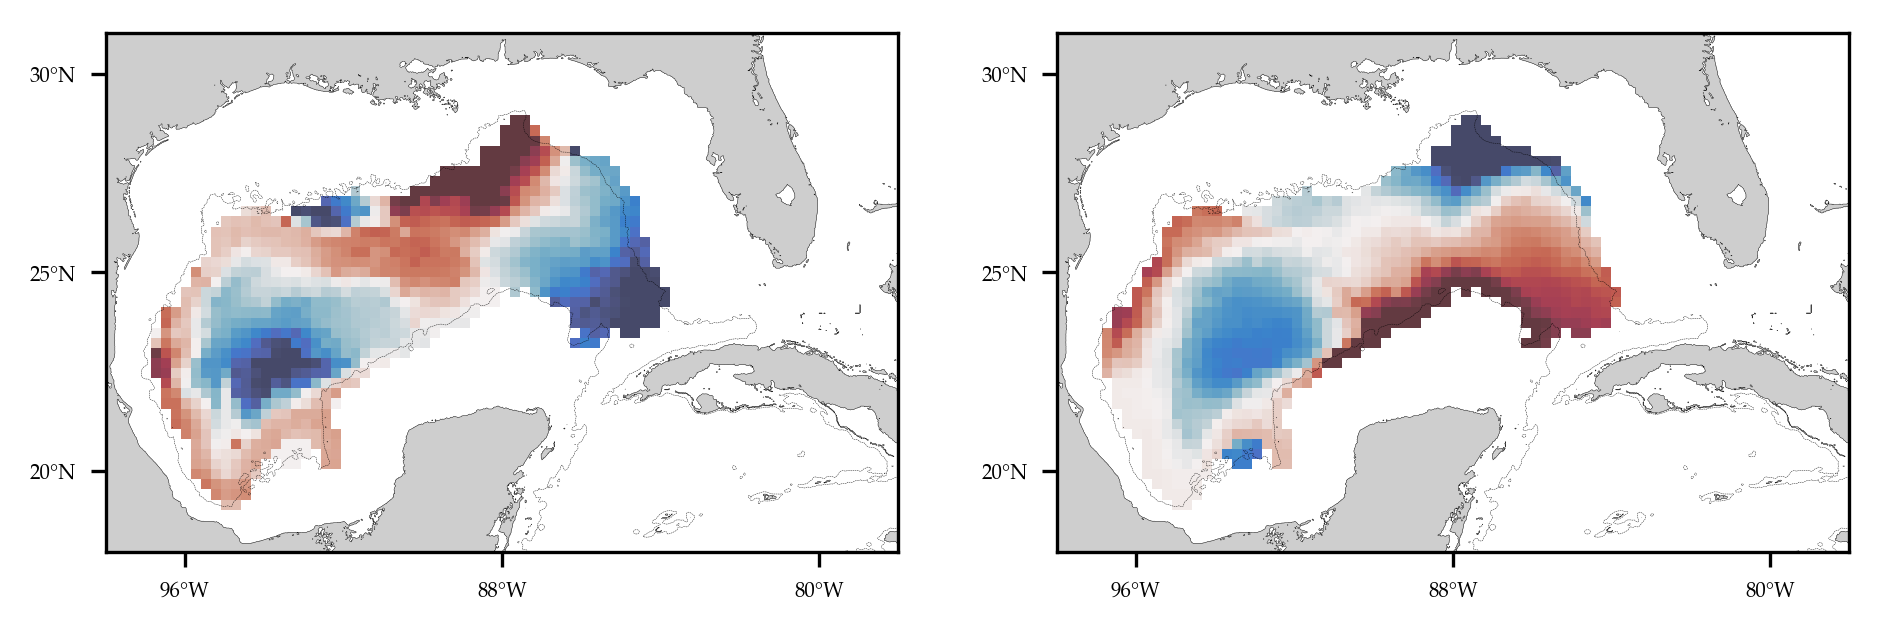
\includegraphics[width=\textwidth]{eig_QP4.png}
\end{figure}
}
}

\frame{\frametitle{Lagrangian geography of the deep Golf of Mexico}

Combination of the basins of attraction from the top right eigenvectors (by thresholding).
\begin{figure}
  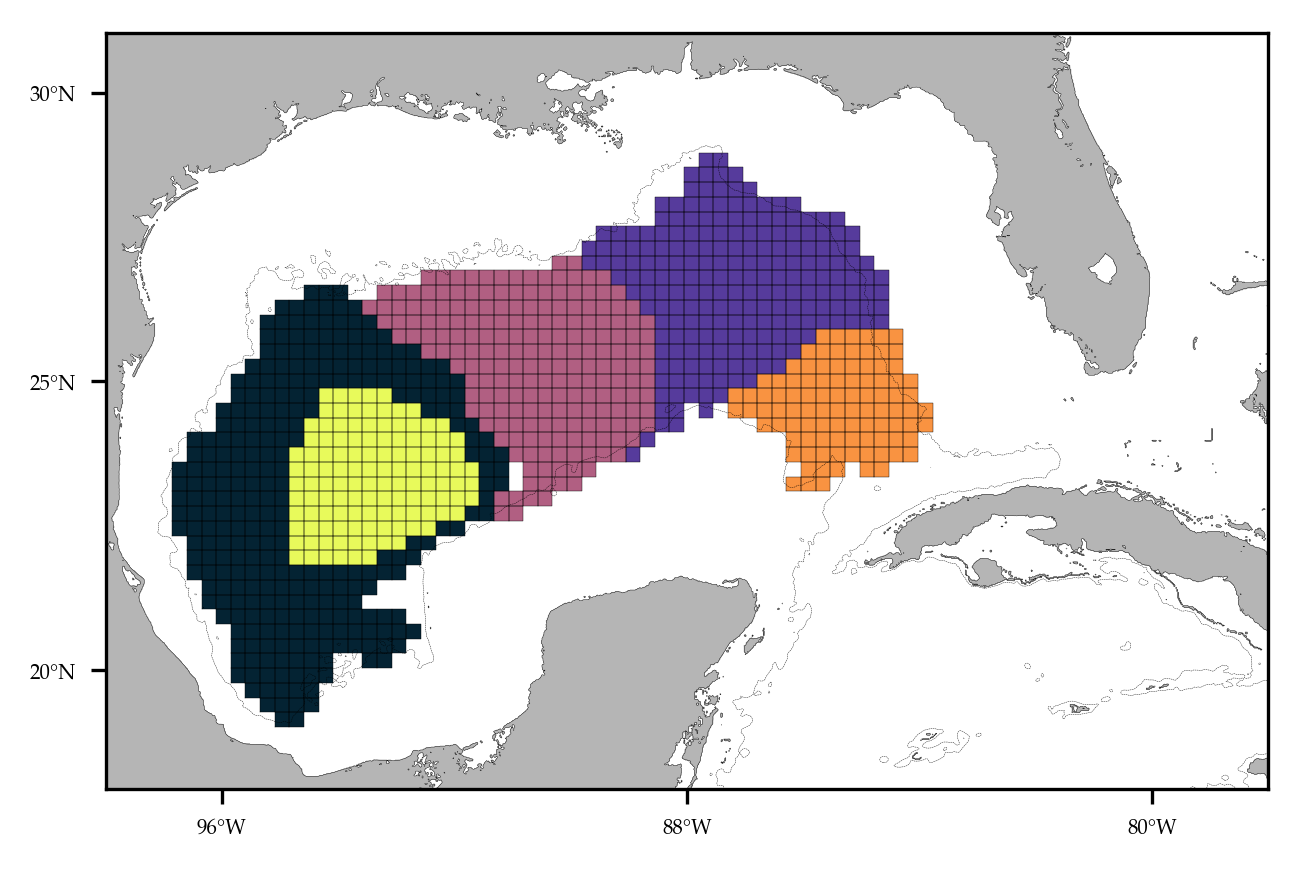
\includegraphics[width=8.5cm]{geodeep.png}
\end{figure}

Residence timescale: 7-y left (black) and right (purple), 1-y middle (pink), 0.5-y gyre (yellow) and bottom right (orange)
}

\frame{\frametitle{Upwelling and Downwelling}
From incompressibility, accumulation can be used to approximate vertical velocity $w$:
\begin{equation}
    h_{t_1} = h_{t_0} \frac{\vol_{t_0}}{\vol_{t_1}} \quad w \sim \frac{h_{t_1} - h_{t_0}}{dt}. 
\end{equation}

\begin{figure}
  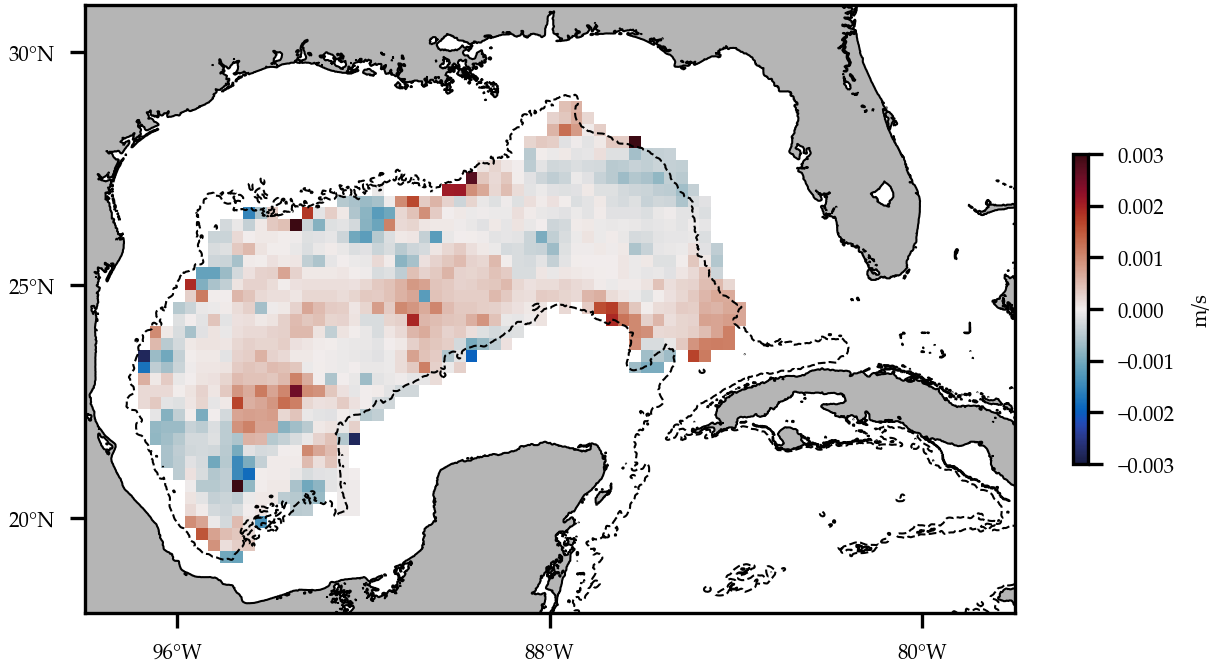
\includegraphics[width=8.5cm]{w.png}
\end{figure}

The vertical component is about $\sim 1\%$ of the maximum horizontal velocity ($u_{max} = 0.2739$m/s, $v_{max} = 0.1790$m/s).
}

\frame{\frametitle{Comparison with experimental data \citep{ledwell2016dispersion}}

\only<1>{
Tracer evolution from the infamous Deepwater Horizon oil spill.
\begin{figure}
  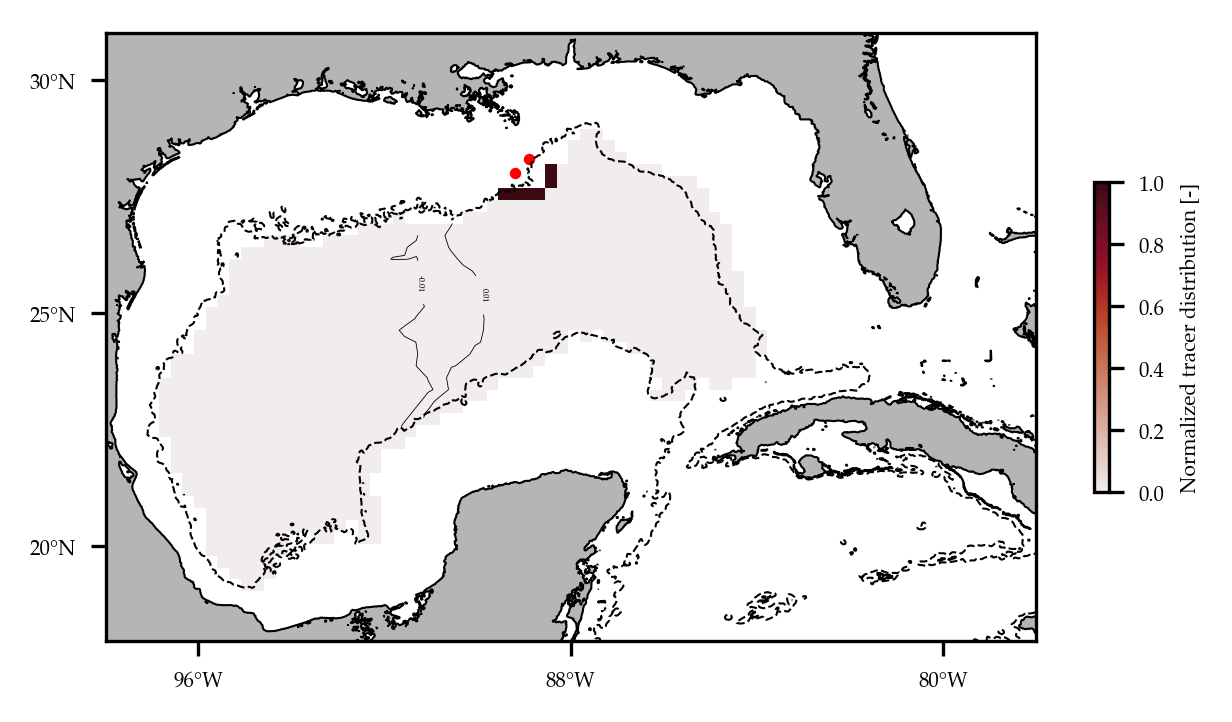
\includegraphics[width=\textwidth]{densityComp-Q-0m.png}
  \caption{Initial location of the tracers}
\end{figure}
}

\only<2>{
\begin{figure}
  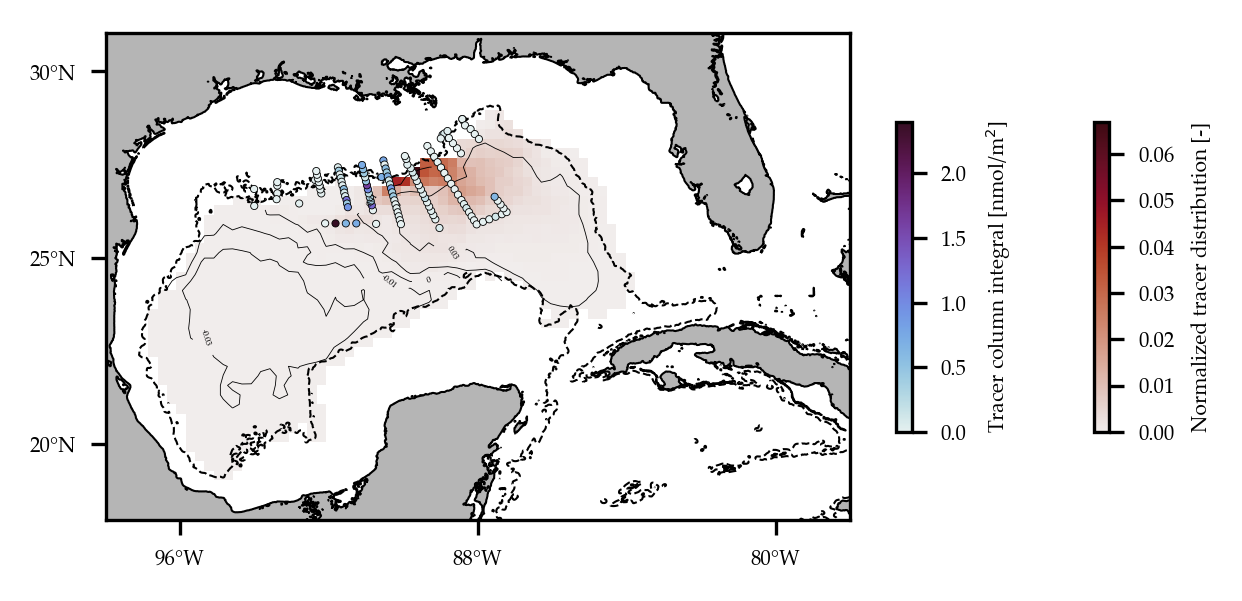
\includegraphics[width=\textwidth]{densityComp-Q-4m.png}
  \caption{Evolution after 4 months}
\end{figure}
}

\only<3>{
\begin{figure}
  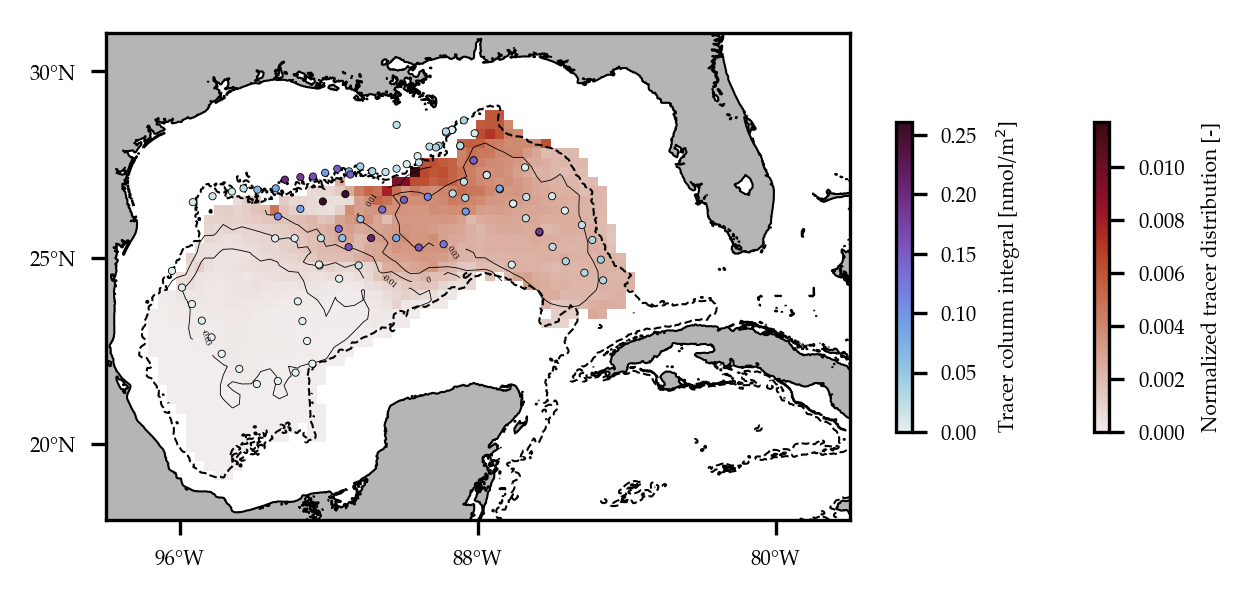
\includegraphics[width=\textwidth]{densityComp-Q-12m.png}
  \caption{Evolution after 12 months}
\end{figure}
}
}

\section{Conclusion}
\frame{\frametitle{Thank you!}

Future plans:
\begin{itemize}
	\item plastic sources and convergence zones
	\item take account inertial effects (see next talk!)
\end{itemize}

Any questions?
}

\frame[allowframebreaks]{\frametitle{References}

% remove References title
\begingroup
\renewcommand{\section}[2]{}%
% add cited papers
\printbibliography[heading=none]
\endgroup
}

\end{document}